% Fixed data array
\def\inputdata{{
    {0, 4, 1, 0},
    {5, 1, 9, 5},
    {3, 6, 7, 3},
    {0, 4, 1, 0}
}}

\def\kerneldata{{
    {2, 3},
    {1, 6}
}}

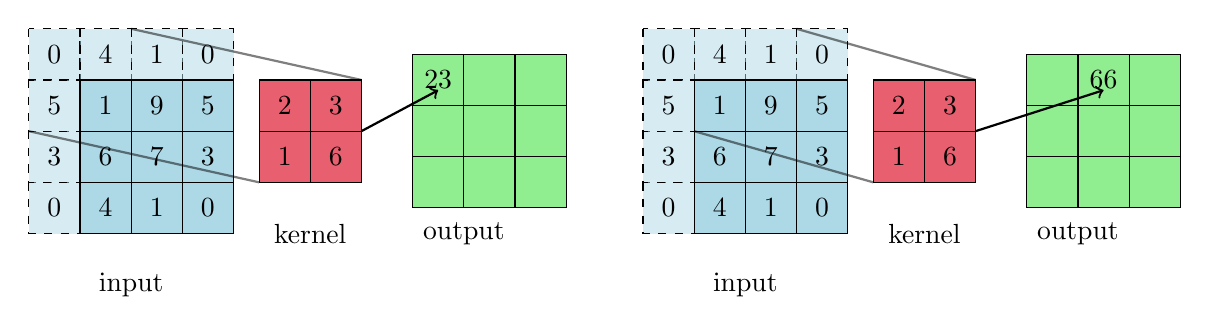
\begin{tikzpicture}[scale=0.65]
\definecolor{inputcolor}{RGB}{173,216,230}
\definecolor{kernelcolor}{RGB}{232,95,111}

% Offsets
\def\xoffset{0}
\def\yoffset{0}

% Draw grid and numbers
\foreach \col in {0,...,3} {
    \foreach \row in {0,...,3} {
        % Get value from array (PGF math arrays are zero-based)
        \pgfmathparse{\inputdata[\row][\col]}
        \let\cellvalue\pgfmathresult

        % Check if first row or first column
        \ifnum\row=0
            \def\cellopacity{0.5}
            \def\cellstyle{dashed}
        \else
            \ifnum\col=0
                \def\cellopacity{0.5}
                \def\cellstyle{dashed}
            \else
                \def\cellopacity{1}
                \def\cellstyle{solid}
            \fi
        \fi

        % Draw at shifted position
        \fill[inputcolor,opacity=\cellopacity] (\xoffset+\col,\yoffset-\row) rectangle ++(1,-1);
        \draw[\cellstyle] (\xoffset+\col,\yoffset-\row) rectangle ++(1,-1);

        % Place number centered in shifted position
        \node at (\xoffset+\col+0.5,\yoffset-\row-0.5) {\cellvalue};
    }
}

\foreach \col in {0,...,1} {
    \foreach \row in {0,...,1} {
        % Get value from array (PGF math arrays are zero-based)
        \pgfmathparse{\kerneldata[\row][\col]}
        \let\cellvalue\pgfmathresult

        % Draw at shifted position
        \fill[kernelcolor] (4.5+\col,-1-\row) rectangle ++(1,-1);
        \draw (4.5+\col,-1-\row) rectangle ++(1,-1);

        % Place number centered in shifted position
        \node at (4.5+\col+0.5,-1-\row-0.5) {\cellvalue};
    }
}

\draw[opacity=0.5,thick] (2,0) -- (6.5,-1);
\draw[opacity=0.5,thick] (0,-2) -- (4.5,-3);

\definecolor{outputcolor}{RGB}{144,238,144}

\foreach \col in {0,...,2} {
    \foreach \row in {0,...,2} {
        \fill[outputcolor] (7.5+\col,-0.5-\row) rectangle ++(1,-1);
        \draw (7.5+\col,-0.5-\row) rectangle ++(1,-1);
        % Add number 23 in the first square
        \ifnum\col=0
            \ifnum\row=0
            \node at (7.5+0.5,-0.5-0.5) {23};
            \fi
        \fi
        }
    }

    \draw[->,thick] (6.5,-2) -- (8,-1.2);

    % Draw a second input grid to the right
    \foreach \col in {0,...,3} {
        \foreach \row in {0,...,3} {
            \pgfmathparse{\inputdata[\row][\col]}
            \let\cellvalue\pgfmathresult

            % Check if first row or first column
            \ifnum\row=0
                \def\cellopacity{0.5}
                \def\cellstyle{dashed}
            \else
                \ifnum\col=0
                    \def\cellopacity{0.5}
                    \def\cellstyle{dashed}
                \else
                    \def\cellopacity{1}
                    \def\cellstyle{solid}
                \fi
            \fi

            \fill[inputcolor,opacity=\cellopacity] (12+\col,\yoffset-\row) rectangle ++(1,-1);
            \draw[\cellstyle] (12+\col,\yoffset-\row) rectangle ++(1,-1);
            \node at (12+\col+0.5,\yoffset-\row-0.5) {\cellvalue};
        }
    }

    % Draw a second kernel grid to the right
    \foreach \col in {0,...,1} {
        \foreach \row in {0,...,1} {
            \pgfmathparse{\kerneldata[\row][\col]}
            \let\cellvalue\pgfmathresult
            \fill[kernelcolor] (16.5+\col,-1-\row) rectangle ++(1,-1);
            \draw (16.5+\col,-1-\row) rectangle ++(1,-1);
            \node at (16.5+\col+0.5,-1-\row-0.5) {\cellvalue};
        }
    }

    \draw[opacity=0.5,thick] (15,0) -- (18.5,-1);
    \draw[opacity=0.5,thick] (13,-2) -- (16.5,-3);

    % Draw a second output grid to the right
    \foreach \col in {0,...,2} {
        \foreach \row in {0,...,2} {
            \fill[outputcolor] (19.5+\col,-0.5-\row) rectangle ++(1,-1);
            \draw (19.5+\col,-0.5-\row) rectangle ++(1,-1);
            % Add number 66 in the second square
            \ifnum\col=1
                \ifnum\row=0
                \node at (19.5+1+0.5,-0.5-0.5) {66};
                \fi
            \fi
        }
    }

    \draw[->,thick] (18.5,-2) -- (21,-1.2);
    % Labels under grids
    \node at (2,-5) {input};
    \node at (5.5,-4) {kernel};
    \node at (8.5,-4) {output};

    \node at (14,-5) {input};
    \node at (17.5,-4) {kernel};
    \node at (20.5,-4) {output};

\end{tikzpicture}